```latex
\chapter{Implementación Secuencial}

La implementación secuencial constituye la línea base (\textit{baseline}) del proyecto y representa la versión de referencia utilizada para validar el correcto funcionamiento del algoritmo antes de desarrollar las versiones paralelas. Todos los experimentos realizados con OpenMP, MPI, CUDA y Multiprocessing fueron comparados contra esta implementación para verificar la consistencia de los resultados obtenidos.

Esta implementación corresponde al Nivel 1 de la arquitectura propuesta para el proyecto de Computación de Alto Rendimiento y ejecuta el algoritmo completo utilizando un único hilo de procesamiento. Su principal propósito consiste en proporcionar una referencia confiable tanto para la validación funcional como para la evaluación del desempeño de las versiones paralelas.

El código fuente principal se encuentra en:

\begin{center}
\texttt{code/secuencial/sequential.py}
\end{center}

\section{Objetivo}

La versión secuencial tiene como propósito ejecutar el algoritmo completo utilizando un único hilo de procesamiento, permitiendo:

\begin{itemize}

\item Validar la exactitud del algoritmo.

\item Obtener una línea base de desempeño.

\item Comparar los resultados de las implementaciones paralelas.

\item Detectar errores antes de introducir mecanismos de paralelización.

\end{itemize}

\section{Descripción General}

La implementación secuencial ejecuta una estrategia de búsqueda aleatoria (\textit{Random Search}) sobre un conjunto de $K$ candidatos pertenecientes al espacio de búsqueda definido por el simplex de pesos.

Cada candidato se genera mediante una distribución de Dirichlet, garantizando automáticamente el cumplimiento de las restricciones:

\[
W_1+W_2+W_3=1,
\qquad
W_i\ge0.
\]

Para cada vector de pesos generado se calcula el perfil ponderado, posteriormente el \textit{score} de todas las muestras y finalmente el valor de la métrica ROC-AUC. Si el candidato evaluado mejora el mejor resultado obtenido hasta ese momento, el algoritmo actualiza la solución óptima.

Todas las evaluaciones se realizan de forma completamente secuencial, sin emplear múltiples procesos ni múltiples hilos de ejecución.

La implementación fue desarrollada en Python utilizando principalmente las bibliotecas \texttt{NumPy} para el procesamiento numérico y \texttt{scikit-learn} para el cálculo de la métrica ROC-AUC.

\section{Flujo de Ejecución}

La Figura \ref{fig:flujo_secuencial} resume el flujo seguido por la implementación secuencial.

\begin{figure}[H]
\centering
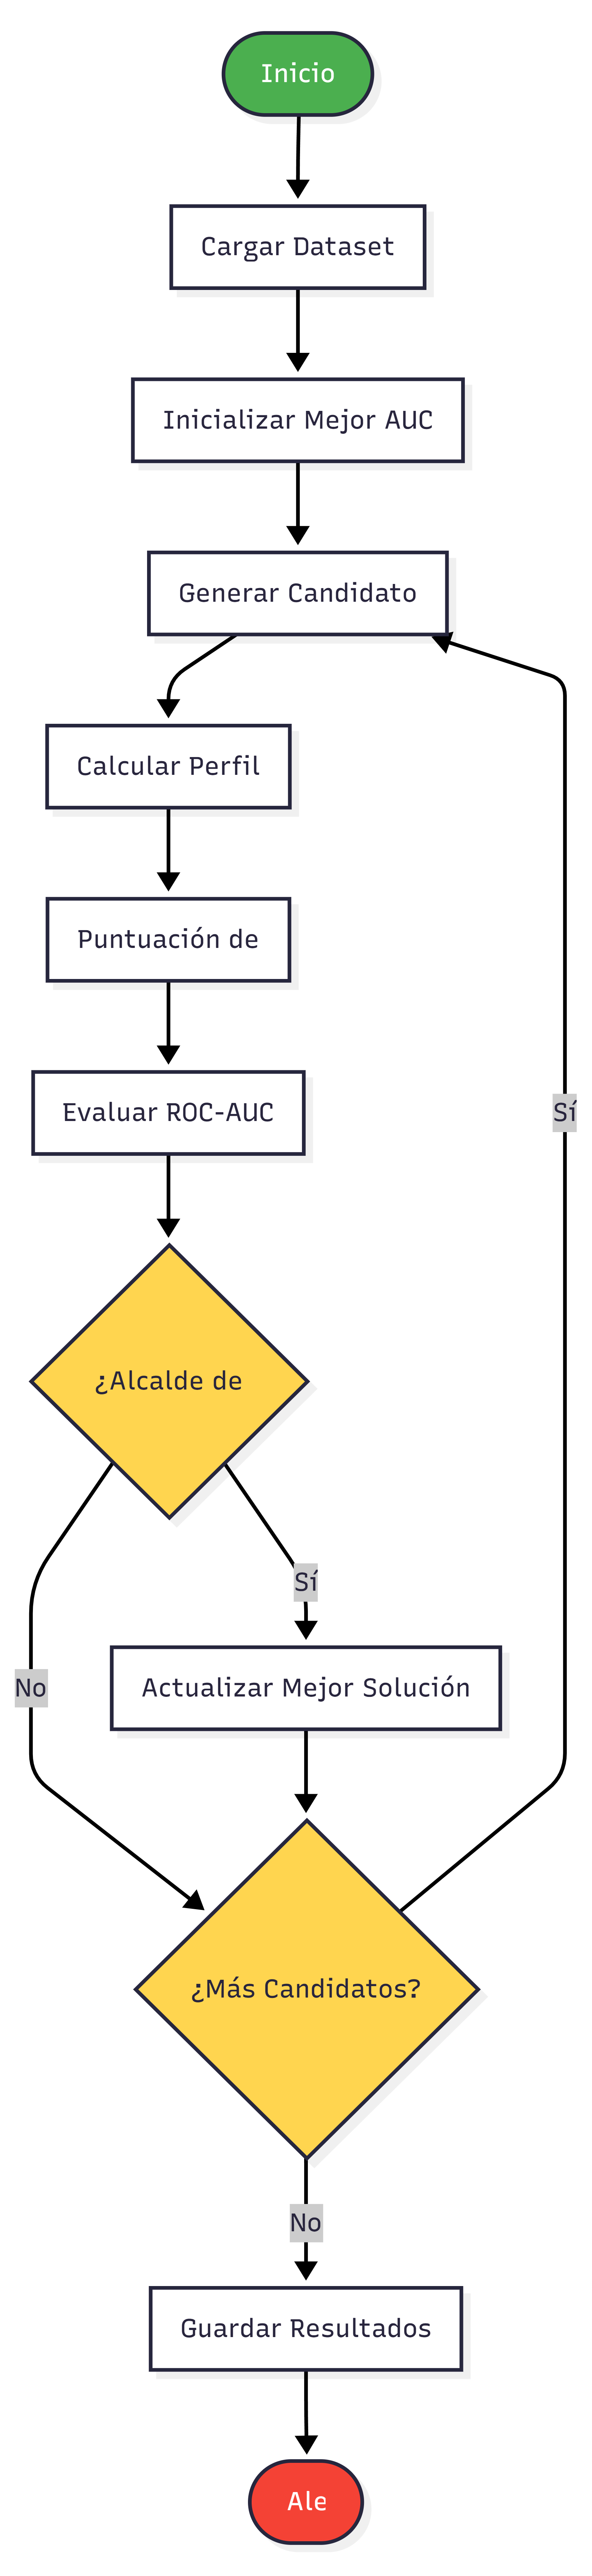
\includegraphics[width=.82\textwidth,height=0.5\textheight,keepaspectratio]
{figuras/implementaciones/01_flujo_secuencial.png}
\caption{Flujo de ejecución de la implementación secuencial.}
\label{fig:flujo_secuencial}
\end{figure}

El procesamiento sigue las siguientes etapas:

\begin{enumerate}

\item Cargar la matriz de datos $A$ y el vector de etiquetas $y$.

\item Inicializar las variables de control.

\item Generar $K$ vectores de pesos candidatos sobre el simplex.

\item Para cada candidato:

\begin{enumerate}

\item Calcular el perfil ponderado.

\item Obtener el \textit{score} correspondiente.

\item Evaluar la métrica ROC-AUC.

\item Comparar el resultado con la mejor solución encontrada.

\end{enumerate}

\item Retornar el mejor vector de pesos encontrado.

\item Registrar las métricas experimentales.

\end{enumerate}

\section{Arquitectura de la Implementación}

La Figura \ref{fig:arquitectura_secuencial} muestra la organización lógica de la implementación secuencial.

\begin{figure}[H]
\centering

\includegraphics[width=.95\textwidth,height=0.5\textheight,keepaspectratio]
{figuras/implementaciones/02_arquitectura_secuencial.png}
\caption{Arquitectura lógica de la implementación secuencial.}
\label{fig:arquitectura_secuencial}
\end{figure}

La implementación está compuesta por un flujo lineal de procesamiento donde cada etapa depende del resultado de la etapa anterior. Esta organización facilita la comprensión del algoritmo y sirve como referencia para las versiones paralelas.

\section{Estrategia de Búsqueda}

El espacio de soluciones se explora mediante una estrategia de búsqueda aleatoria (\textit{Random Search}). En cada iteración se genera un nuevo vector de pesos perteneciente al simplex utilizando una distribución de Dirichlet.

Cada candidato representa una solución completamente independiente de las demás, lo que permite que la lógica del algoritmo permanezca inalterada cuando posteriormente se distribuyen las evaluaciones entre múltiples procesos o hilos en las implementaciones paralelas.

Durante toda la ejecución únicamente se conserva el candidato con mayor valor de ROC-AUC, evitando almacenar resultados intermedios y manteniendo un bajo consumo de memoria.

\section{Pseudocódigo}

El procedimiento implementado puede resumirse mediante el siguiente pseudocódigo.

\begin{lstlisting}
cargar_datos(A, y)

mejor_auc = 0

para candidato = 1 hasta K

    generar_pesos_simplex()

    calcular_perfil()

    score = A * P

    auc = calcular_ROC_AUC(score)

    si auc > mejor_auc

        actualizar_mejor_solucion()

fin

guardar_resultados()
\end{lstlisting}

\section{Complejidad Computacional}

Sea:

\begin{itemize}

\item $K$: número de candidatos.

\item $N$: número de características.

\item $M$: número de muestras.

\end{itemize}

Cada candidato debe recorrer completamente el conjunto de datos para calcular el perfil ponderado y posteriormente evaluar la métrica ROC-AUC.

La complejidad temporal aproximada puede expresarse como

\[
O(K \times N \times M)
\]

mientras que el consumo de memoria permanece aproximadamente constante durante toda la ejecución, puesto que únicamente se conserva el mejor candidato encontrado.

Dado que la evaluación de cada candidato es completamente independiente del resto, esta complejidad constituye el punto de partida para las implementaciones paralelas desarrolladas en el proyecto, cuyo objetivo consiste en reducir el tiempo efectivo de ejecución distribuyendo la evaluación de los candidatos entre múltiples unidades de procesamiento.

\section{Ventajas}

La implementación secuencial presenta diversas ventajas:

\begin{itemize}

\item Simplicidad de desarrollo.

\item Fácil depuración.

\item Bajo nivel de complejidad.

\item Resultados completamente deterministas para una misma semilla.

\item Referencia utilizada para validar todas las implementaciones paralelas.

\end{itemize}

\section{Limitaciones}

Entre las principales limitaciones se encuentran:

\begin{itemize}

\item No aprovecha procesadores multinúcleo.

\item Incremento lineal del tiempo de ejecución.

\item Baja escalabilidad para grandes volúmenes de datos.

\item Elevados tiempos de procesamiento cuando aumenta el número de candidatos.

\end{itemize}

Estas limitaciones motivan el desarrollo de las implementaciones paralelas descritas en los capítulos posteriores.

\section{Evidencia Experimental}

La Figura \ref{fig:ejecucion_secuencial} presenta una ejecución de muestra de la implementación secuencial durante los experimentos realizados.

\begin{figure}[H]
\centering
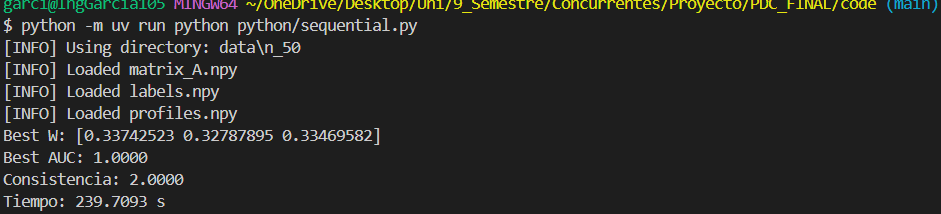
\includegraphics[width=.95\textwidth,height=0.45\textheight,keepaspectratio]
{figuras/capturas/secuencial.png}
\caption{Ejecución de muestra de la implementación secuencial.}
\label{fig:ejecucion_secuencial}
\end{figure}

Las Figuras \ref{fig:secuencial_prueba_01} a \ref{fig:secuencial_prueba_05} presentan los resultados de las pruebas experimentales realizadas.

\begin{figure}[H]
\centering
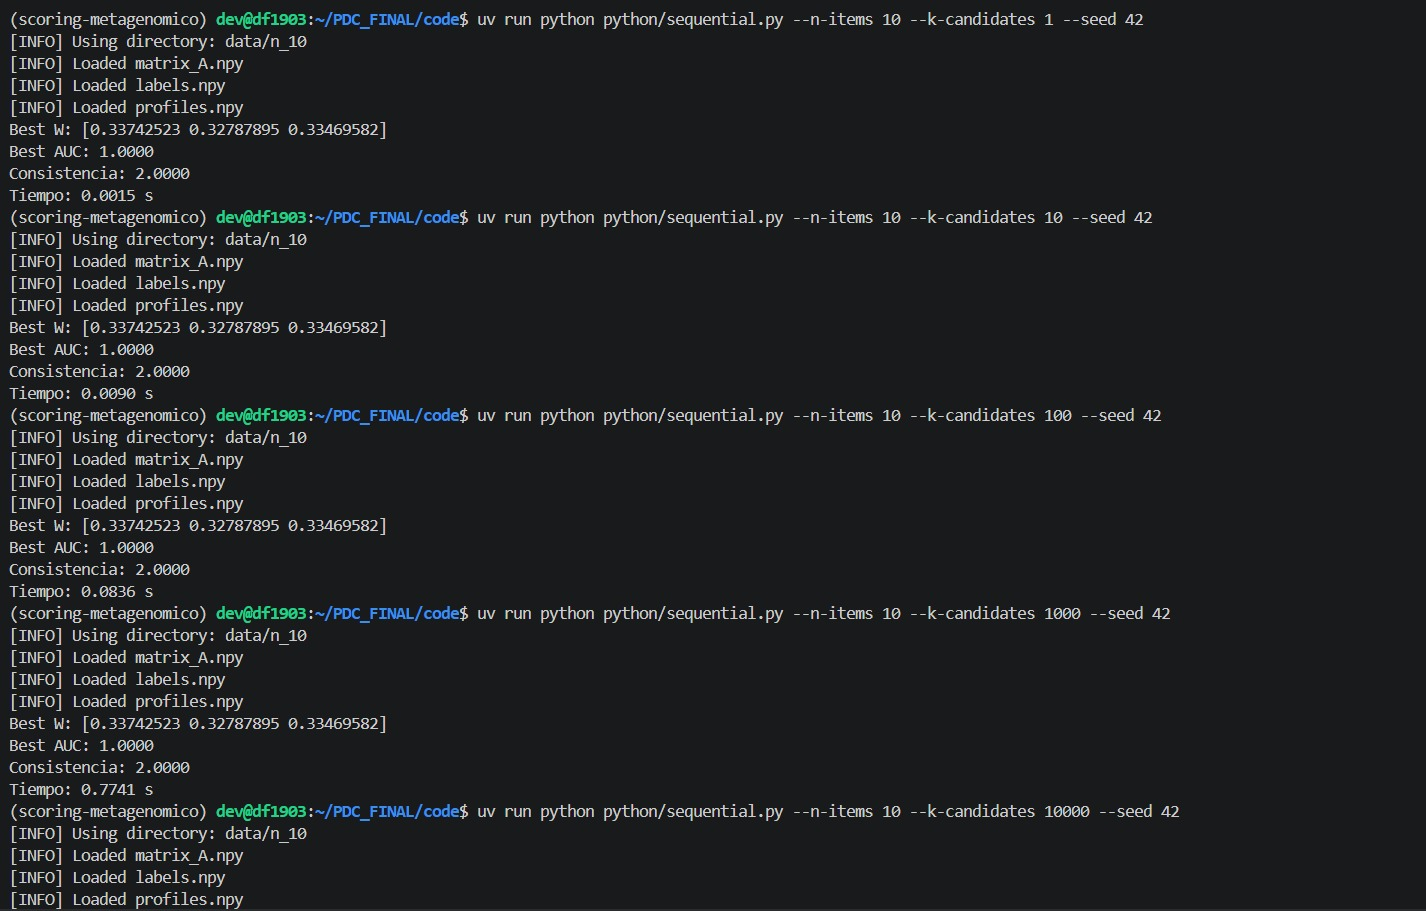
\includegraphics[width=.95\textwidth,height=0.45\textheight,keepaspectratio]
{figuras/capturas/secuencial_01.png}
\caption{Prueba experimental 1 -- Implementación secuencial.}
\label{fig:secuencial_prueba_01}
\end{figure}

\begin{figure}[H]
\centering
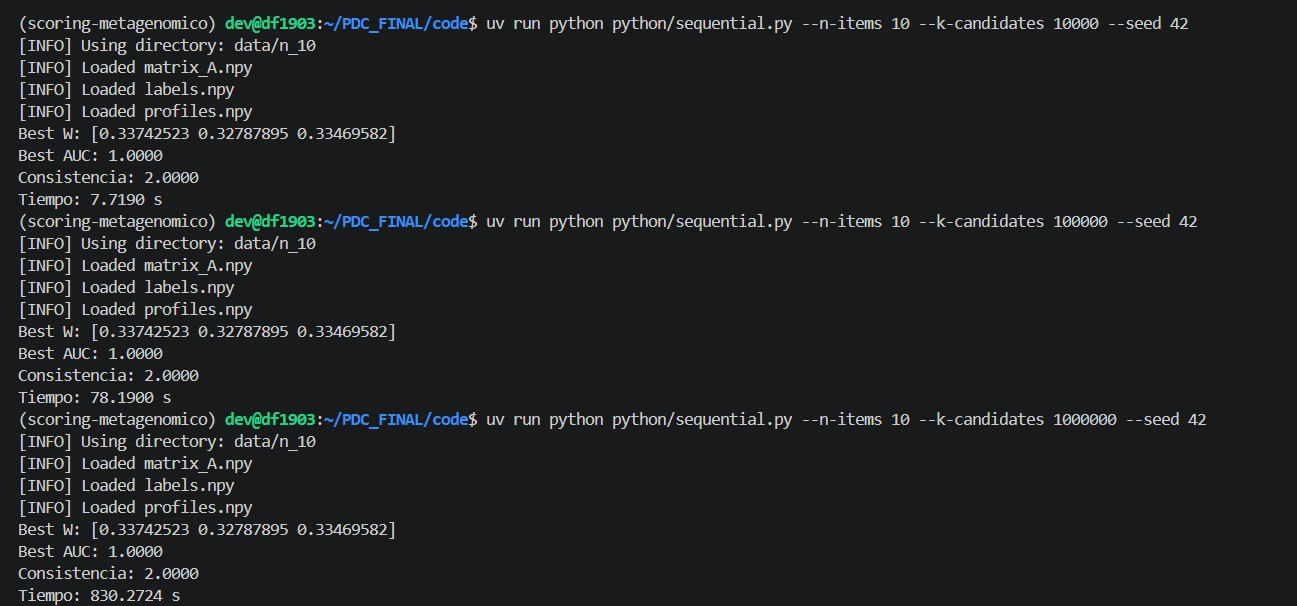
\includegraphics[width=.95\textwidth,height=0.45\textheight,keepaspectratio]
{figuras/capturas/secuencial_02.png}
\caption{Prueba experimental 2 -- Implementación secuencial.}
\label{fig:secuencial_prueba_02}
\end{figure}

\begin{figure}[H]
\centering
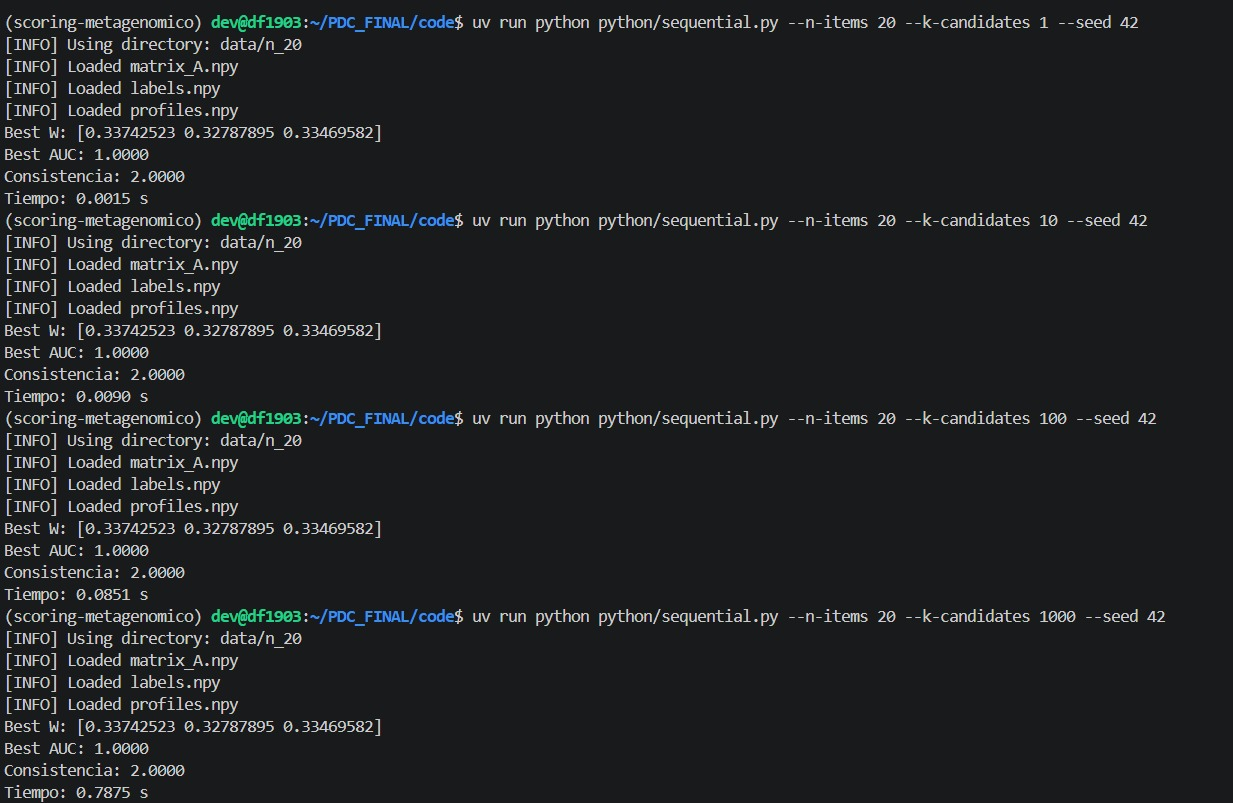
\includegraphics[width=.95\textwidth,height=0.45\textheight,keepaspectratio]
{figuras/capturas/secuencial_03.png}
\caption{Prueba experimental 3 -- Implementación secuencial.}
\label{fig:secuencial_prueba_03}
\end{figure}

\begin{figure}[H]
\centering
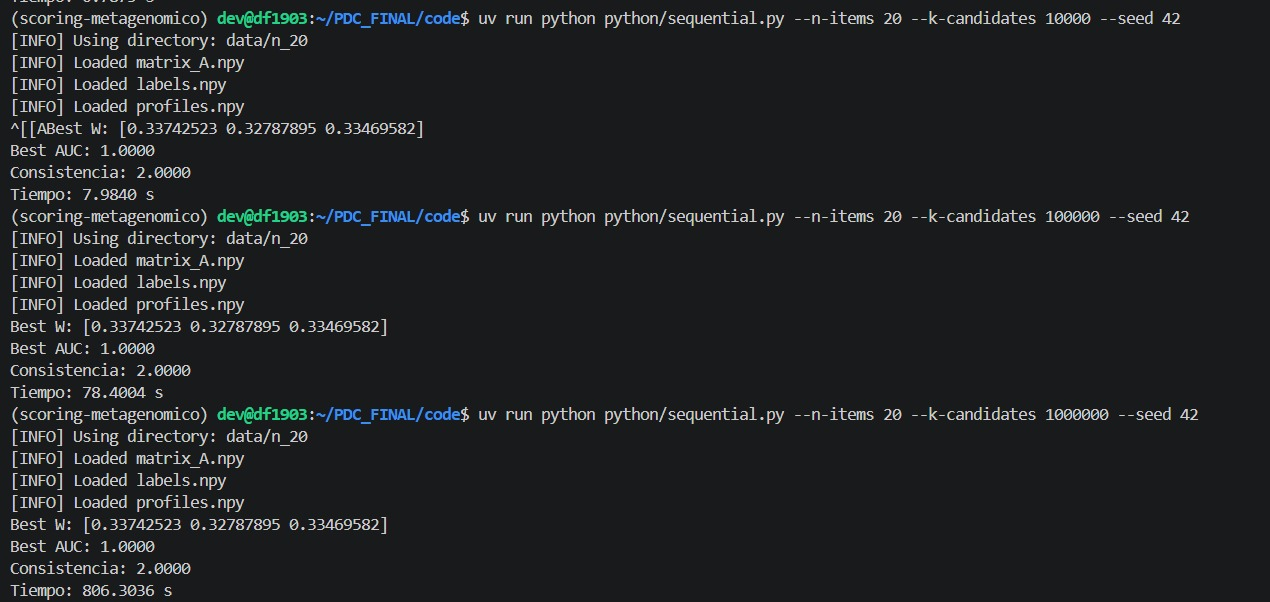
\includegraphics[width=.95\textwidth,height=0.45\textheight,keepaspectratio]
{figuras/capturas/secuencial_04.png}
\caption{Prueba experimental 4 -- Implementación secuencial.}
\label{fig:secuencial_prueba_04}
\end{figure}

\begin{figure}[H]
\centering
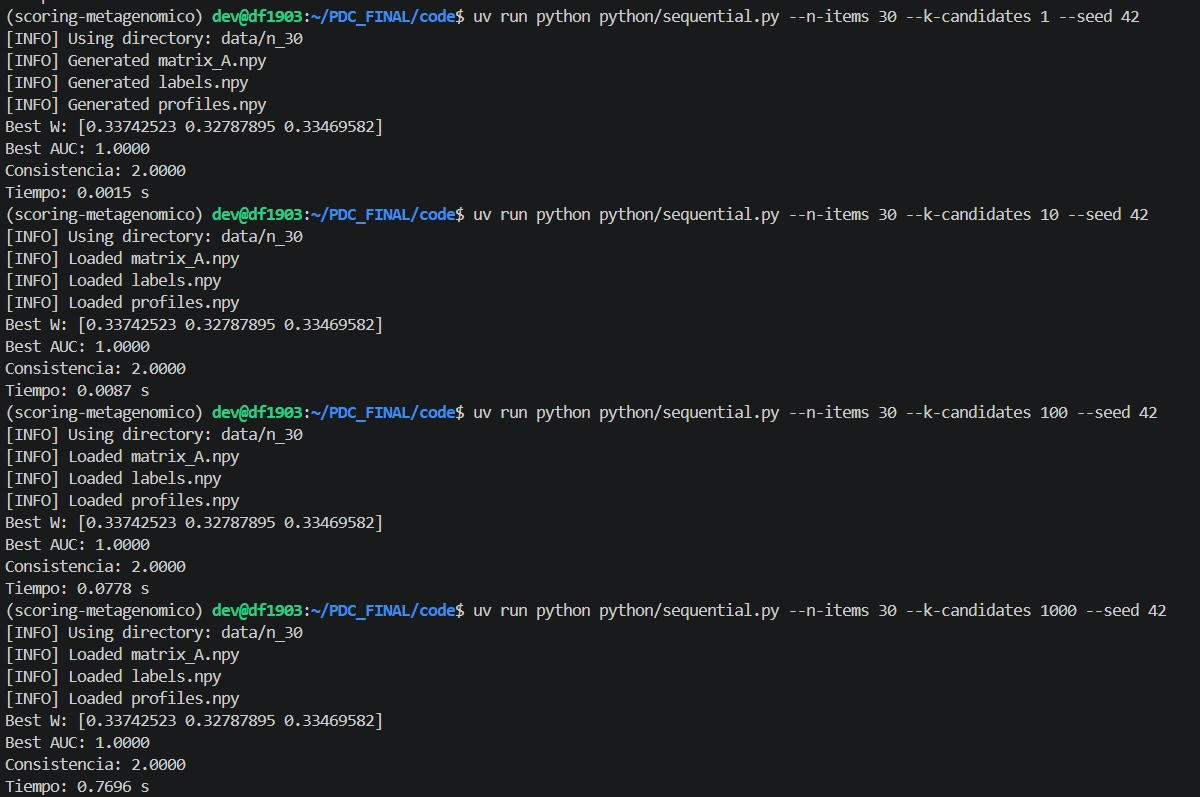
\includegraphics[width=.95\textwidth,height=0.45\textheight,keepaspectratio]
{figuras/capturas/secuencial_05.png}
\caption{Prueba experimental 5 -- Implementación secuencial.}
\label{fig:secuencial_prueba_05}
\end{figure}

Durante la ejecución se registran automáticamente el tiempo total de procesamiento, el mejor valor de ROC-AUC obtenido, el vector de pesos óptimo y el número total de candidatos evaluados.

Estos resultados constituyen la línea base utilizada posteriormente para calcular las métricas de Speedup, Eficiencia y realizar la comparación de desempeño entre las diferentes estrategias de paralelización desarrolladas en el proyecto.
```
